\documentclass{article}
\usepackage[margin=1.0in]{geometry}
\usepackage{graphicx}
\graphicspath{{./img}}
\title{Image Processing Homework 3: Image Compression}
\author{Andr\'es Ponce \\
\and
0616110}
\date{\today}

\begin{document}
\maketitle
\section{Introduction}
Image compression is a task with tremendous importance in the modern world. Countless numbers
of images, videos, movies and other visual  content are shared every day. Wihtout a way to reduce 
the memory usage of this content, long-term storage would be impractical and the cost of storing
such media would be impractical. A single image with $1920\times1080$ resolution would consume

\[1920 \times 1080 \times 3 \times 8 = 49,766,400 \textrm{ bytes}\]

There are various image compression algorithms and standards which allow the easy sharing of such 
content. Among them is the JPEG compression method, which utilizes many of the methodologies 
introduced in the textbook. In this report, the following techniques are introduced: Huffman coding,
predictive coding, discrete cosine transform.

These methods are implemented in Python and then compared to see the amount of saved storage they 
allow us to achieve.

\section{Methods}
\subsection{Huffman Coding}
Huffman coding remains one of the most famous compression techniques.  This technique finds a 
variable length code such that the most used symbols in our message are assigned the shortest
codes. We first calculate the probability of each symbol in the set. We then make a tree by 
joining the two elements with the lowest probability under a single parent with combined
probability. We repeat this procedure until we are left with a single node of probability 1.

This method proves optimal because the lengths of the symbols increases as their frequency
decreases. Huffman coding results in a nearly optimal method. Once we have a string with which
to encode a message, once converted into a binary format it becomes easier to format. The 
set of strings will most likely be shorter. In my implementation, the strings with the lowest
frequency tended to be much longer on average. 

In my experiment, most of the strings ended up being between 3 and 6 bits in length. Since greyscale
images were used, this average would be a considerable saving over a definite 8 bytes per pixel.
In the decoding stage, we only have to search the tree for the corresponding intensity to that
string. 
\subsection{Discrete Cosine Transform}
Similar to the Discrete Fourier Transform, this method decomposes a signal as a combination
of trigonometric functions, however the DCT only uses a combination of cosine and scalar
values to compress a signal. The formula used in this assignment is 
\[f(x, y, u, v) = \alpha_{u}\alpha_{v}\sum_{u=1}^{B}\sum_{v=1}^{B}\cos{\frac{(2x+1)u\pi}{2B}} \
\cos{\frac{(2y+1)v\pi}{2B}}\]

where $B$ is the block size, which was left to 8 in this assignment.

The implementation was straightforward, however the transformed image contained quite 
small values. These were extremely tiny values, mostly exponentials with exponent -14
or -15. With this rough implementation it would lead to promising results if a suitable
code were chosen for the frequency values.

\subsection{Predictive Coding}
With predictive coding, we attempt to exploit the similarity in adjacent pixels. We have a
predicted value $e(n)$, and we attempt to add it with the sum of previous $m$ samples to 
obtain our estimate. The formula used in this assignment was 

\[f(x, y) = e(n) + \hat{f}(x, y)\]
where $e(n)$ is the difference between the current pixel and the current pixel, $\hat{f}(x, y)$.
Specifically, $\hat{f}(x, y)$ is defined as 
\[2f(x, y) - f(x-1, y) - f(x, y-1)\]
i.e. we take the difference with the pixel in the previous row and column.

This method, if combined also with a variable length code technique, could also provide a much shorter
encoding that 8 bits used for greyscale values. A method such as Huffman could provide a more 
efficient method than just saving the different smaller integer.

\subsection{Run-Length Coding}
The main purpose of this type of coding is to reduce many repeated pixel values that are next to each other. 
For example, if there is a background in an image many pixels might have the exact same value in case of the 
sky or some building. If we somehow store the value of the pixel and how many consecutive pixels have the 
same value, we could avoid storing multiple copies of the same value. For example, a tuple with the 
values (180, 3) would indicate that the following 3 pixels each are of intensity 180.

This coding method can be used to great efficacy when dealing with the raw binary values. BMP files 
use this compression method as mentioned in the textbook, and for binary images it would probably have 
the best effect. 

\section{Code}
Following are screenshots from the main code section of each of the methods.
\subsection{Huffman}
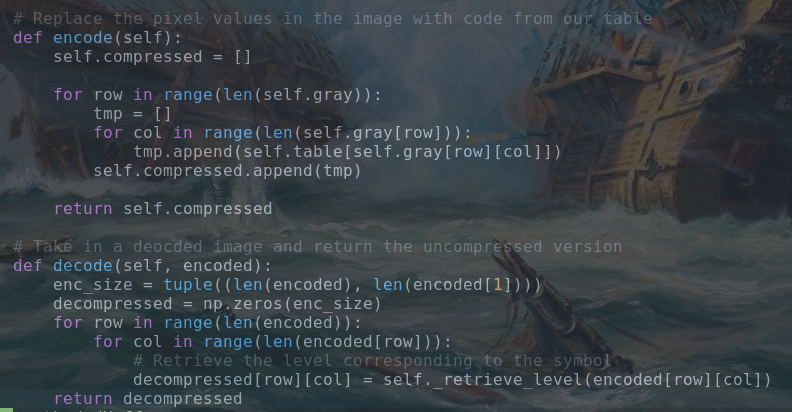
\includegraphics[scale=.40]{huff1.png}


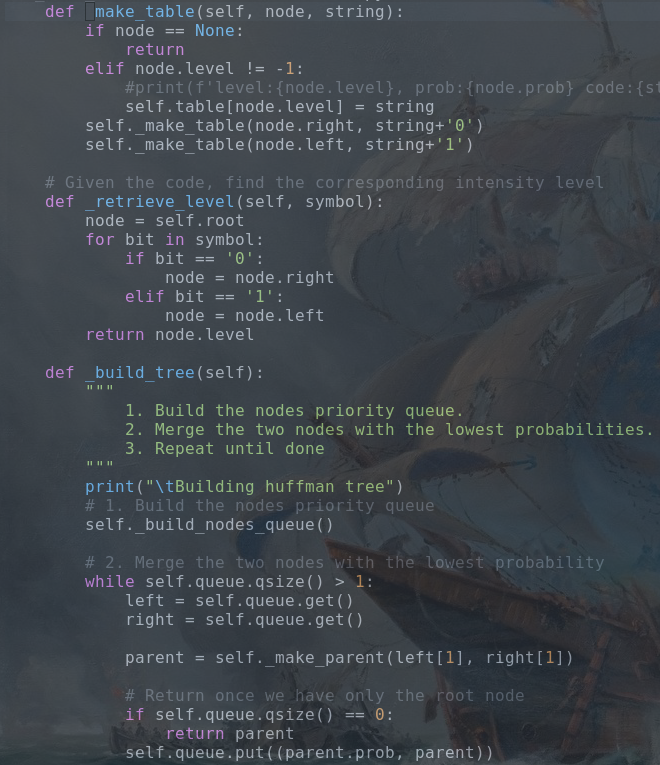
\includegraphics[scale=.40]{huff2.png}

These two images show the main functions of the Huffman coding procedure: building the 
tree and getting the frequencies, inserting them into the tree, and then decoding the 
image.

\subsection{Discrete Cosine Transform}
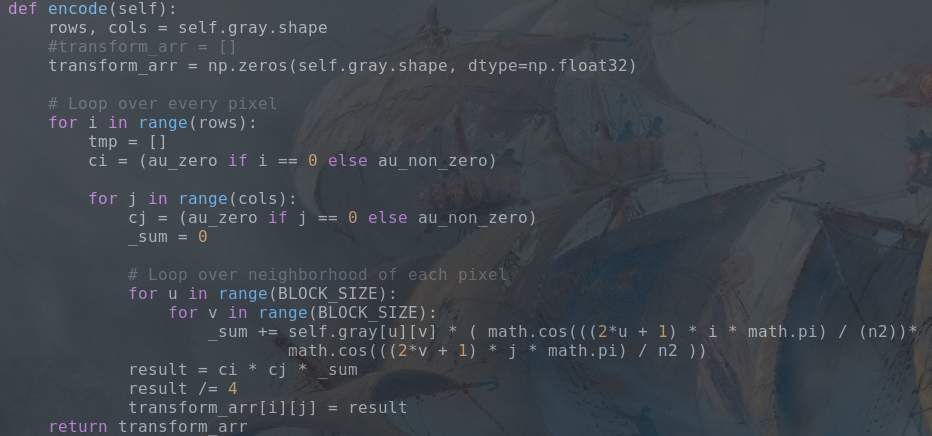
\includegraphics[scale=.50]{dct1.png}

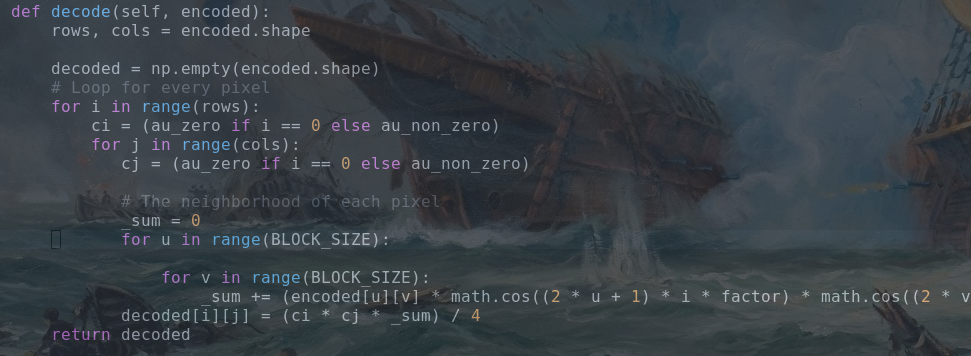
\includegraphics[scale=.50]{dct2.png}
%
\subsection{Predictive Coding}
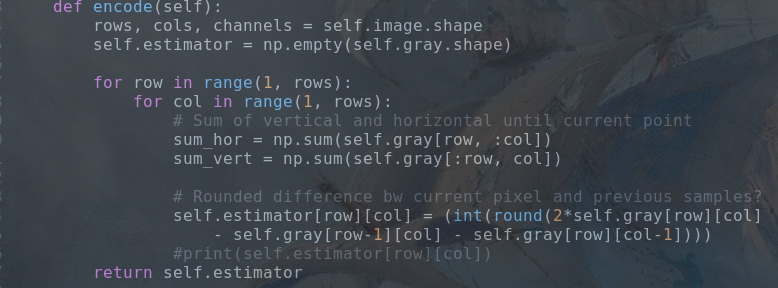
\includegraphics[scale=.60]{pred1.png}

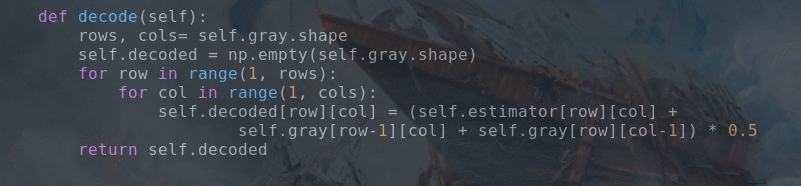
\includegraphics[scale=.60]{pred2.png}

\subsection{Run-Length Coding}
%
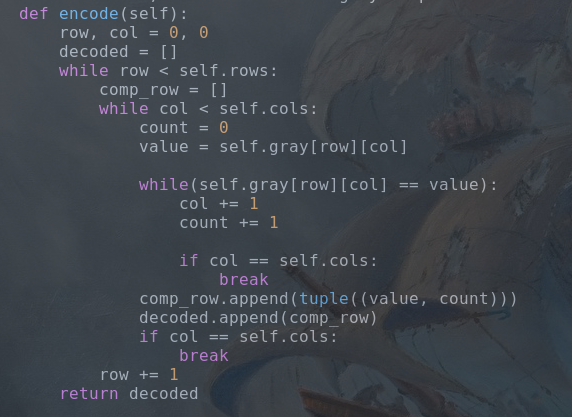
\includegraphics[scale=.60]{rlc1.png}

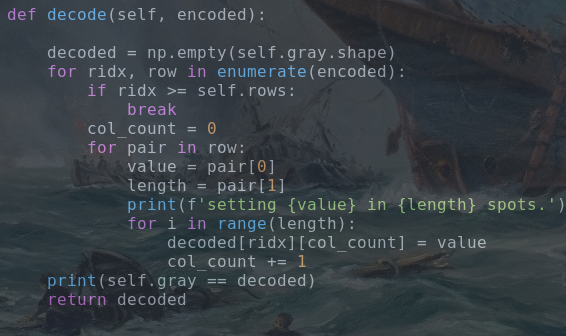
\includegraphics[scale=.60]{rlc2.png}
\end{document}
